\documentclass{article}

\usepackage{geometry}
\geometry{
  a4paper,
  total={170mm,257mm},
  left=20mm,
  top=20mm,
}

\usepackage{cite}
\usepackage{kotex}
\usepackage{float}
\usepackage{amsmath,amssymb,amsfonts}
\usepackage[ruled, vlined]{algorithm2e}
\usepackage{graphicx}
\usepackage{textcomp}
\usepackage{xcolor}
\usepackage{listings}
\usepackage{caption}
\usepackage{subcaption}
\usepackage{multirow}
\usepackage{booktabs}
\usepackage{makecell}
\usepackage{hyperref}
\hypersetup{
    colorlinks=true,
    linkcolor=blue,
    filecolor=magenta,
    urlcolor=cyan,
}
\urlstyle{same}

\lstset{basicstyle=\ttfamily}

\begin{document}

\title{$\textsf{JUSTGen}$: Effective Test Generation for Unspecified JNI Behaviors on JVMs
\\ {\large Artifact Evaluation}}

\author{
  Sungjae Hwang
  \and
  Sungho Lee
  \and
  Jihoon Kim
  \and
  Sukyoung Ryu
}
\date{KAIST, South Korea}

\maketitle

\section{Artifact Description}

\begin{figure}[H]
  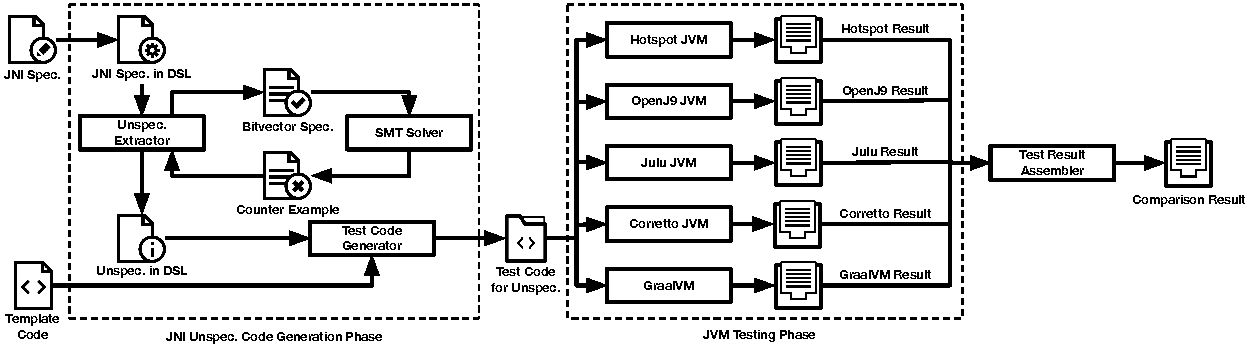
\includegraphics[width=0.98\textwidth]{dsl_overview3.pdf}
\end{figure}

JUSTGen is a framework that consists of two parts. The first part identifies unspecified cases from the JNI specification expressed in our DSL (Domain Specific Language). The second part generates test programs triggering the behaviors of the identified unspecified cases. The artifact consists of following modules:

\begin{itemize}
  \item \textbf{Unspec. Extractor} finds unspecified cases from the JNI specification expressed in our DSL. 
  \item \textbf{Test Code Generator} generates test programs triggering identified unspecified cases
  
\end{itemize}


\section{Getting Started Guide}

The artifact is open-source can be obtained by cloning the following git
repository:
\begin{lstlisting}
$ git clone https://github.com/sjmini/justgen.git 
\end{lstlisting}
To build and execute the artifact, you should follow the instrucitons in the
\texttt{INSTALL} file in the artifact. 
The instructions of how to build and execute the tool are also summarized in the above git repository

For convenience, we packaged the artifact in a vm image.
All the neccessary sw packages are installed in this vm image.
The tester only need to clone the artifact and build it through make command.
The ID and PW for the VM image are as follow:

ID: justgen

PW: 1234

\end{document}
